\documentclass{standalone}
\usepackage{tikz}

\begin{document}

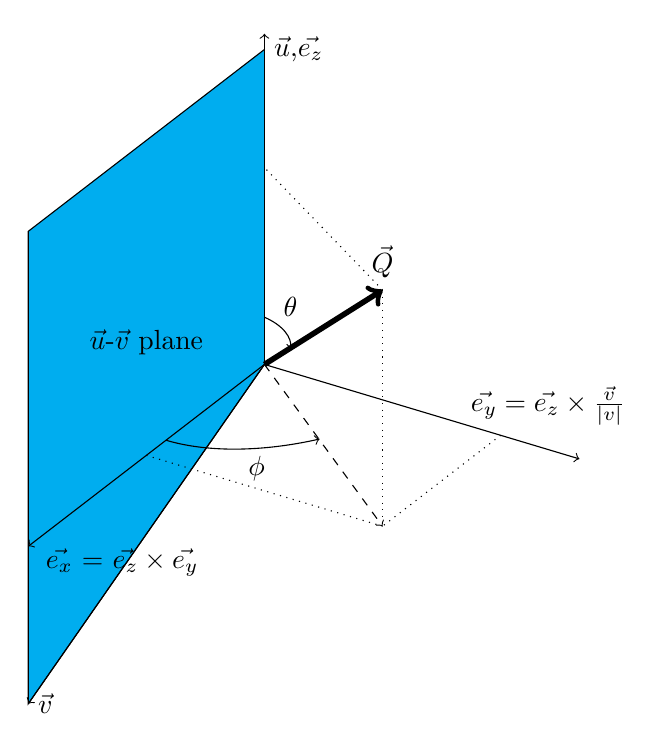
\begin{tikzpicture}[x={(-5mm,-3.85mm)},z={(0,1cm)},y={(1cm,-.3cm)}]
  \draw [fill=cyan] (0,0,0)--(6,0,-2)--(6,0,4)--(0,0,4) node [above, xshift=-1.5cm,yshift=-4cm] {$\vec{u}$-$\vec{v}$ plane};

  \draw [->] (0,0) -- (6,0,-2) node [right] {$\vec{v}$};
  \draw [->] (0,0) -- (0,4,0) node [above,xshift=-0.4cm,yshift=0.3cm] {$\vec{e_y} = \vec{e_z} \times \frac{\vec{v}}{|v|}$};
  \draw [->] (0,0) -- (0,0,4.2) node [right,yshift=-0.2cm] {$\vec{u}$,$\vec{e_z}$};

  \draw [->] (0,0) -- (6,0,0) node [right,xshift=0.1cm,yshift=-0.2cm] {$\vec{e_x}$ = $\vec{e_z} \times \vec{e_y}$};

  \draw [dotted] (3,3,3) -- (0,0,2.5);
  
  \draw [dotted] (0,3,0)  -- (3,3,0);
  \draw [dotted] (3,0,0) -- (3,3,0);  

  \draw [line width=2pt,->] (0,0,0) -- (3,3,3) node [above] {$\vec{Q}$};
  \draw [dotted] (3,3,3) -- (3,3,0);
  \draw [dashed,->] (0,0,0) -- (3,3,0);

  \draw [->] (0,0,0.6) arc [start angle=170,end angle=120,x radius=1.2,y radius=0.9] node [above,yshift=0.3cm] {$\theta{}$};
  \draw [->] (2.5,0,0) arc [start angle=0,end angle=44,x radius=4,y radius=2] node [below,xshift=-0.8cm,yshift=-0.1cm] {$\phi$};

\end{tikzpicture}

\end{document}
